\section{Acceleration calculation}
In the Barnes-Hut algorithm, the net acceleration of a particle $p$ is calculated by summing the contributions from single particles or groups of particles while traversing the tree.
The decision whether the acceleration can be approximated using the information stored in an internal node $n$ depends on the relative distance from $p$ to $n.\textrm{COM}$ (the center of mass of group represented by $n$).
The distance is relative to the \textit{width} $H$ of the node, i.e. the side length of the cubical volume encompassed by the node.
More concretely, the approximation takes place if $n.H / |n.\mathrm{COM} - p.\mathbf{x}| < \theta$, where $\theta$ is the so-called \textit{opening angle}.
In the extreme case when $\theta$ is set to zero, no approximations take place, and the algorithm reduces to the PP method.
The procedure described above is illustrated in \autoref{alg:bh-find-force}.
\begin{algorithm}
    \caption{Compute gravitational force on a particle using Barnes-Hut approximation}
    \label{alg:bh-find-force}
    \begin{algorithmic}[1]
        \Function{FindAcceleration}{$n$, $p$, $\theta$}
        \If{$n$ is an external node}
        \If{$n$ contains a particle $q \neq p$}
        \State $p.\mathbf{a} \gets p.\mathbf{a} + \Call{GravitySoft}{q.\mathbf{x}, q.m, p.\mathbf{x}} / p.\text{mass}$
        \EndIf
        \State \Return
        \EndIf
        \If{$n.H / |n.\text{COM} - p.\mathbf{x}| < \theta$}
        \State $p.\mathbf{a} \gets p.\mathbf{a} + \Call{Gravity}{n.\mathrm{COM}, n.M, p.\mathbf{x}}$
        \State \Return
        \EndIf
        \ForAll{child $n_c$ of $n$}
        \State \Call{FindAcceleration}{$n_c$, $p$, $\theta$}
        \EndFor
        \EndFunction
    \end{algorithmic}
\end{algorithm}
In the implementation, the \textsc{GravitySoft} function calculates the gravitational force softened by $\epsilon$, i.e. it returns the value given by \autoref{eq:softened-force}.
The pairwise potential energy associated with this force is given by
\begin{equation}\label{eq:pe-soft}
    \Phi_{ij}^\textrm{soft} = - \frac{G m_i m_j}{\sqrt{r_{ij}^2 + \epsilon^2}}.
\end{equation}
The \textsc{Gravity} function returns the approximation (up to the quadrupole term) of the acceleration due to a group of particles represented by a given node, i.e.
\begin{equation*}
    \mathbf{a} = -GM \frac{\mathbf{r}}{r^3} + \frac{G}{r^5}\mathbf{Q}\mathbf{r} - \frac{5G}{2}(\mathbf{r} \cdot (\mathbf{Q} \mathbf{r})) \frac{\mathbf{r}}{r^7}
\end{equation*}
(see \cite{hernquist1987performance}).

One possible way to quantify the quality of approximation for a given value of $\theta$ is to consider the relative error of calculated force.
We set the same initial conditions of the system for both the PP direct summation method and the Barnes-Hut algorithm, compute the deviation of Barnes-Hut forces from PP forces acting on each particle, and take the average over all particles.
In other words, the error calculated is given by the \autoref{eq:force-avg-relative-err}.
The dependence of the error on the opening angle $\theta$ and the corresponding execution time are shown in \autoref{fig:bh-analysis}.
The figure includes plots for two cases: when only the monopole term is used in the Barnes-Hut approximation, and when both the monopole and quadrupole terms are included.
As can be seen, the quadrupole-based algorithm exhibits significantly improved error scaling with increasing $\theta$.
Naturally, this raises the question of the additional computational cost incurred by the inclusion of the quadrupole term.
Our tests showed that this impact is minimal.
The results (for $N = 10{,}000$ particles and $0 \leq \theta \leq 2$) support this observation.
\begin{figure}[htp]
    \centering
    \begin{subfigure}[b]{0.47\textwidth}
        \centering
        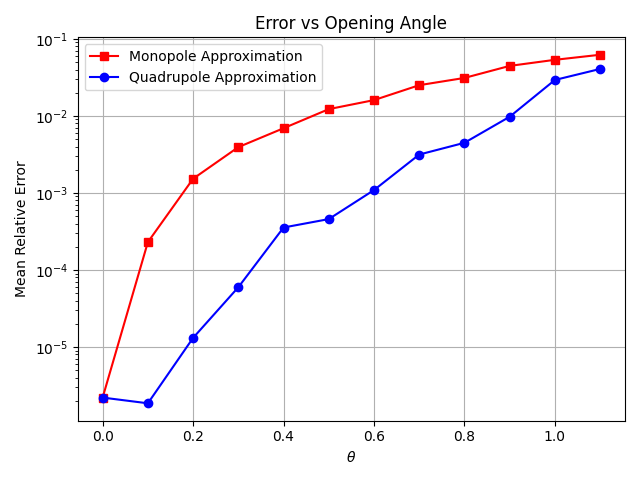
\includegraphics[width=\textwidth]{chapters/barnes-hut/img/error-vs-theta.png}
        \caption{Force approximation error.}
        \label{fig:bh-force-error}
    \end{subfigure}
    \hfill
    \begin{subfigure}[b]{0.47\textwidth}
        \centering
        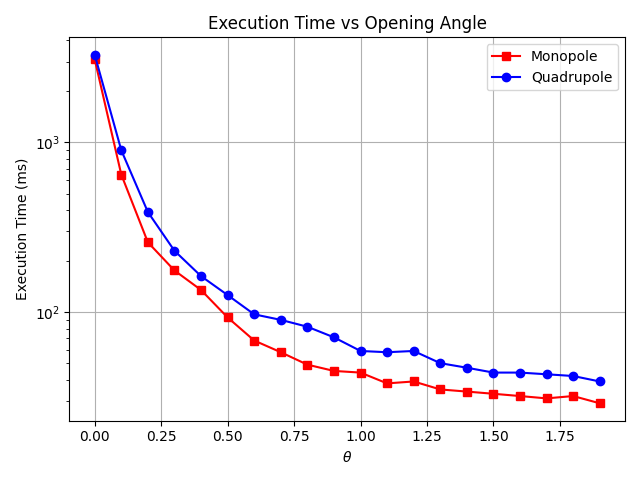
\includegraphics[width=\textwidth]{chapters/barnes-hut/img/bh-time.png}
        \caption{Execution time per iteration.}
        \label{fig:bh-time}
    \end{subfigure}
    \caption{Comparison of error and execution time in the Barnes-Hut algorithm using monopole and quadrupole approximations.}
    \label{fig:bh-analysis}
\end{figure}
Both tests described above were conducted on a uniform disk particle distribution.

We note that direct calculation of total potential energy is infeasible as $O(N^2)$ operations would be required.
Instead, we use an approximation based on the values stored in the tree.
The approximate value of the potential energy is accumulated for each particle using a procedure analogous to force calculation.
Indeed, the only difference between the two is the replacement of gravitational force calculation in \autoref{alg:bh-find-force} with potential energy calculation according to \autoref{eq:pe-soft}.

It is also noteworthy that the procedure outlined in \autoref{alg:bh-find-force} is embarrassingly parallel.
In our CPU implementation, the workload is split between an arbitrary number of threads on particle-by-particle basis.
